\chapter{Evaluation}
This evaluation outlines the process of testing the performance of the localization system using orthogonal codes in underwater environments. The chapter covers the simulation of the system, in which a benchmark is used to assess the performance with different levels of SNR by adding white noise. 

Additionally, the chapter discusses the field testing of the algorithm, which is performed in a real-world scenario using three hydrophones configured as two sending anchors and one receiver. The simulation and field testing results provide valuable insights into the accuracy and reliability of the localization system.
\section{Simulation}
The simulation part involves the use of a Watermark benchmark \cite{watermark15} and the addition of Gaussian white noise with varying levels of signal-to-noise ratio (SNR) to the signals. The simulation then evaluates the performance by following a simulated path of positions in 3D space, using four anchors.
\subsection{Watermark}
The Watermark Simulation consists of a convolution or channel replay by an selected channel TVIR estimate. The channels consist of multiple dirac impulses of different strengths. Thus, reflections and reduced signal strength are simulated.\
\begin{equation}
	x_{tSigTBr}[k]=\sum_{i=0}^{N}h[k,i]\cdot x_{tSigTB}[k-i]
\end{equation}

\subsection{White noise}
A additive Gaussian White Noise (GWN) generated by a desired Signal to Noise Ratio (SNR) between \SI{-20}{\decibel} and \SI{20}{\decibel} in steps of \SI{5}{\decibel}. From the general equation of the Signal to Noise Ratio we derive our noise standard deviation by transforming this ratio. The white noise is added after the simulation and before receiver filtering. To estimate the power of our signal a standard deviation estimation is used, which consists of all incoming signals by using its expected value. The Gaussian noise is generated by using a normal distributed random variable with its mean at zero and its standard deviation at $\frac{\bar{\sigma}}{SNR}$. Thus, $M$ denotes the number of total anchors and $N$ is the length of the corresponding signal.
\begin{equation}	
	\bar{\sigma}=\cfrac{1}{M}\sum_{i=0}^{M}\sigma_i,~~~\sigma_j=\sum_{k=0}^{N}{tSigTBr_j}^2[k]
\end{equation}
\begin{equation}
	n[k]=f_{GWN}[k]\cdot \cfrac{\bar{\sigma}}{SNR},~~~GWN\sim\text{Normal}(0,1)
\end{equation}
\begin{figure}[h]
	\centering
	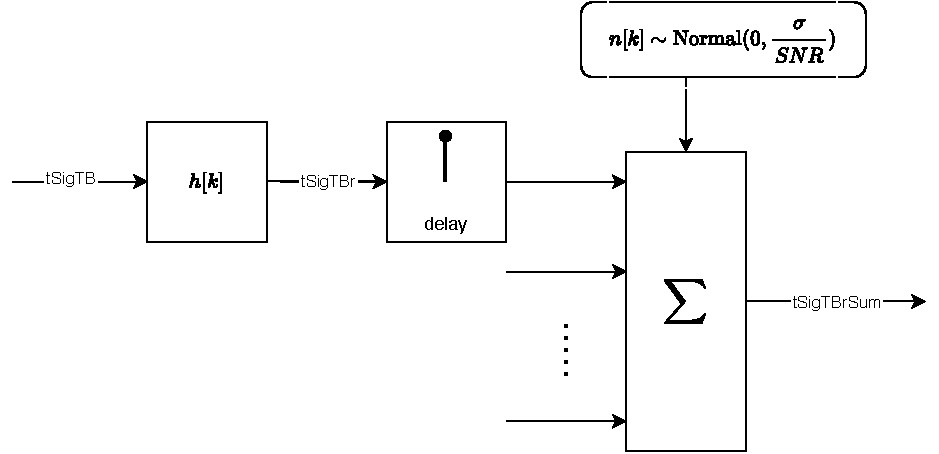
\includegraphics[width=\linewidth]{images/simsig}
	
	\caption{Simulation of acoustic signal underwater propagation}
	\label{fig:simsig}
\end{figure}

\subsection{Localization simulation}
To test the localization algorithm, several 3-dimensional space paths were simulated, wherein the generated points formed a helical curve that expanded in the $z$-direction \ref{eq:helix}. The positions of four anchors were utilized to calculate the TDOA values using multilateration techniques, which were subsequently incorporated into the localization algorithm \ref{eq:dist2toa}. Further, an approximate value of \SI{1500}{\meter\per\second} for the speed of sound $c$ in water was used as a parameter in the calculations. Multiple runs, utilizing varying SNR's and watermark channels were conducted to evaluate the performance of the peak detection method.

\begin{equation}
	\vec{x}_{\phi}(\alpha,\beta)
	=\left[
	\begin{array}{c}
		\alpha\cdot\sin{\phi}+\beta\\
		\alpha\cdot\cos{\phi}+\beta\\
		-|\phi| \leq z \leq -1
	\end{array}
	\right]
	\label{eq:helix}
\end{equation}
\begin{equation}
	\tau_i = \frac{1}{c} \cdot \left(\left| S - S_0 \right | - \left | S - S_i \right|\right)
	\label{eq:dist2toa}
\end{equation}
The simulation system is based on 20 simulated positions. An almost rectangle coverage for the target is created using four anchor coordinates $S_0=(\SI{15}{\meter},\SI{1}{\meter},\SI{17}{\meter})$, $S_1=(\SI{200}{\meter},\SI{10}{\meter},\SI{5}{\meter})$, $S_2=(\SI{195}{\meter},\SI{210}{\meter},\SI{6}{\meter})$ and $S_3=(\SI{16}{\meter},\SI{190}{\meter},\SI{3}{\meter})$ to be located in. The circular curve is scaled by \SI{30}{\meter} and has an offset of \SI{100}{\meter} from the point of origin.  The CA-FAR lower threshold is set to $0.2$ to exclude accidental peak detection in low amplitude correlation phases.

The results of the simulation of position detection indicate that, as the noise level increases and the signal-to-noise ratio decreases, some positions cannot be accurately located \ref{fig:3dvs1}. This intrusion of noise leads to a failure of the peak detection due to new peaks with high similarity to the real ones. The correlations reveal that, with increased noise, the side lobes of the correlation peaks become more prominent, making it difficult to detect peaks \ref{fig:3dvslines1}. Additionally, a higher CFAR threshold, which is a side effect of the additive noise, may result in the rejection of valid peaks.

\begin{figure}
	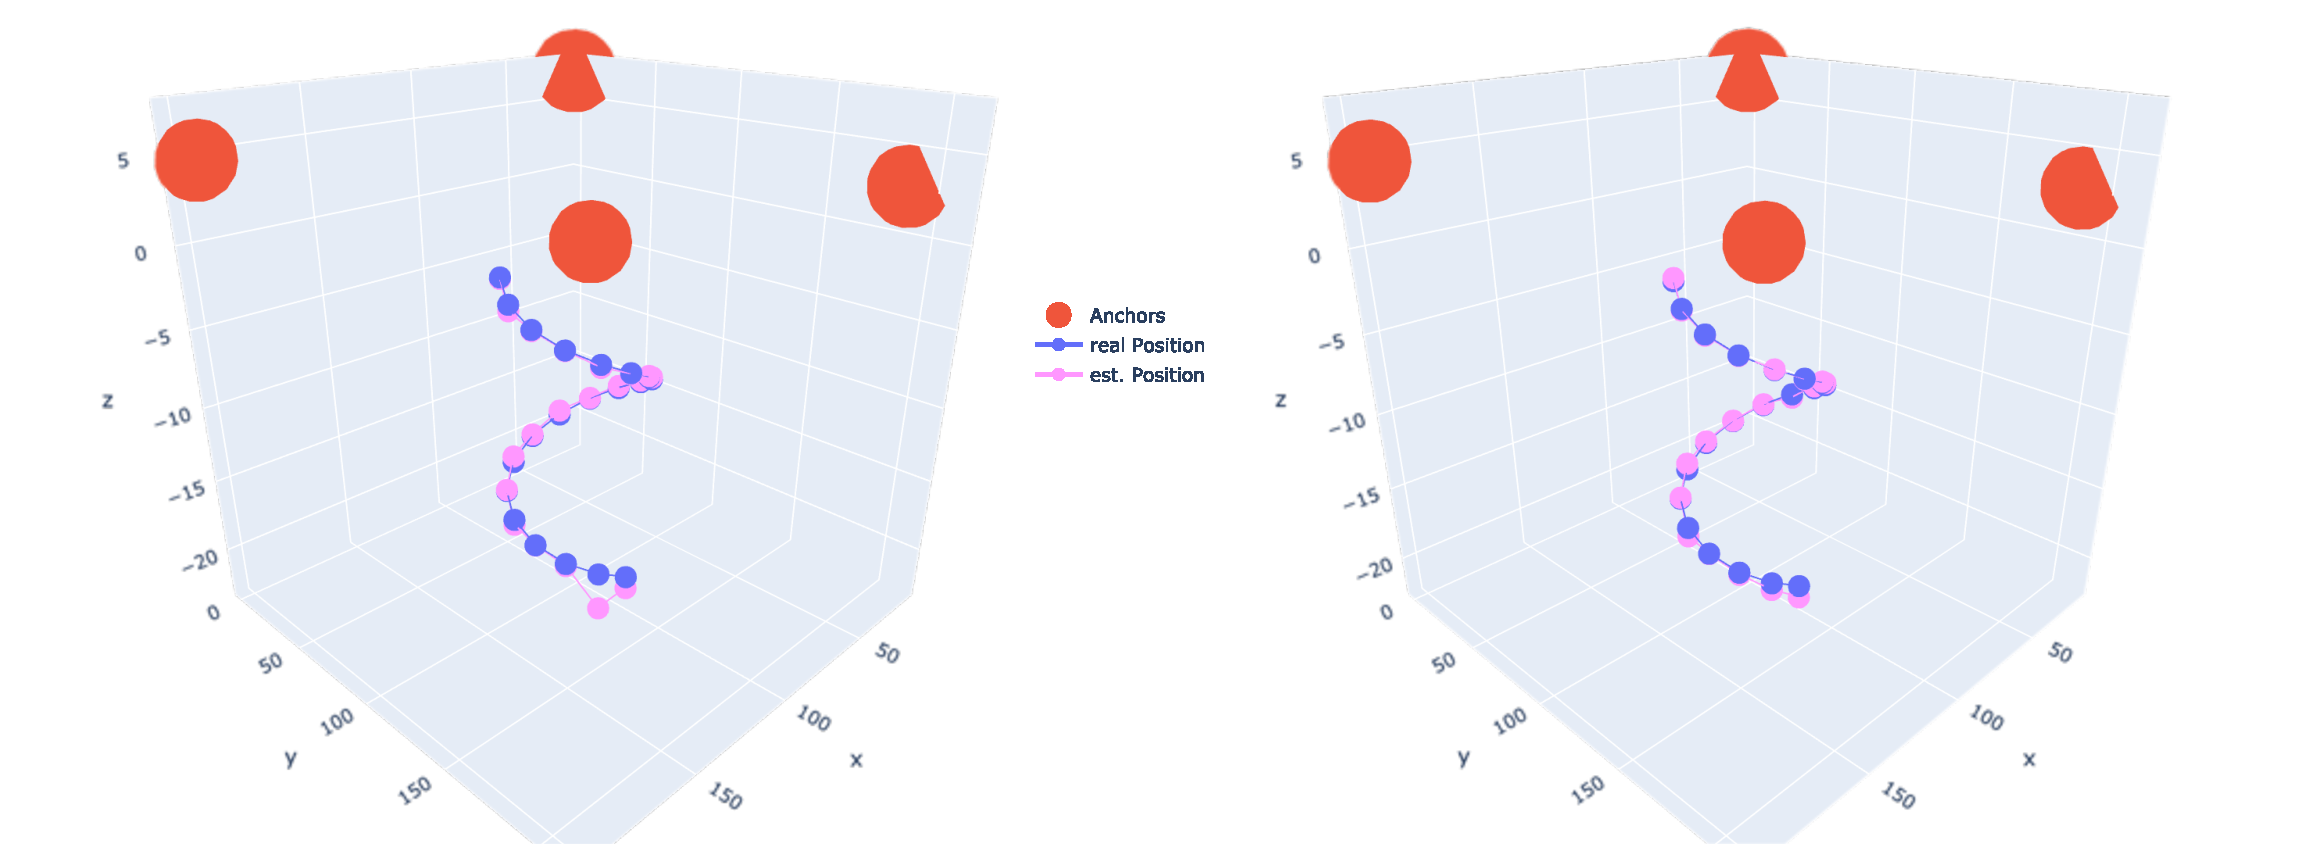
\includegraphics[width=\linewidth]{images/simulation/d10-5snrvs20snr} 
	\caption{3D position evaluation with code of 10th degree. Left one shows \SI{-5}{\decibel} and right one \SI{20}{\decibel} signal strength created by additive noise.}
	\label{fig:3dvs1}
\end{figure}
\begin{figure}
	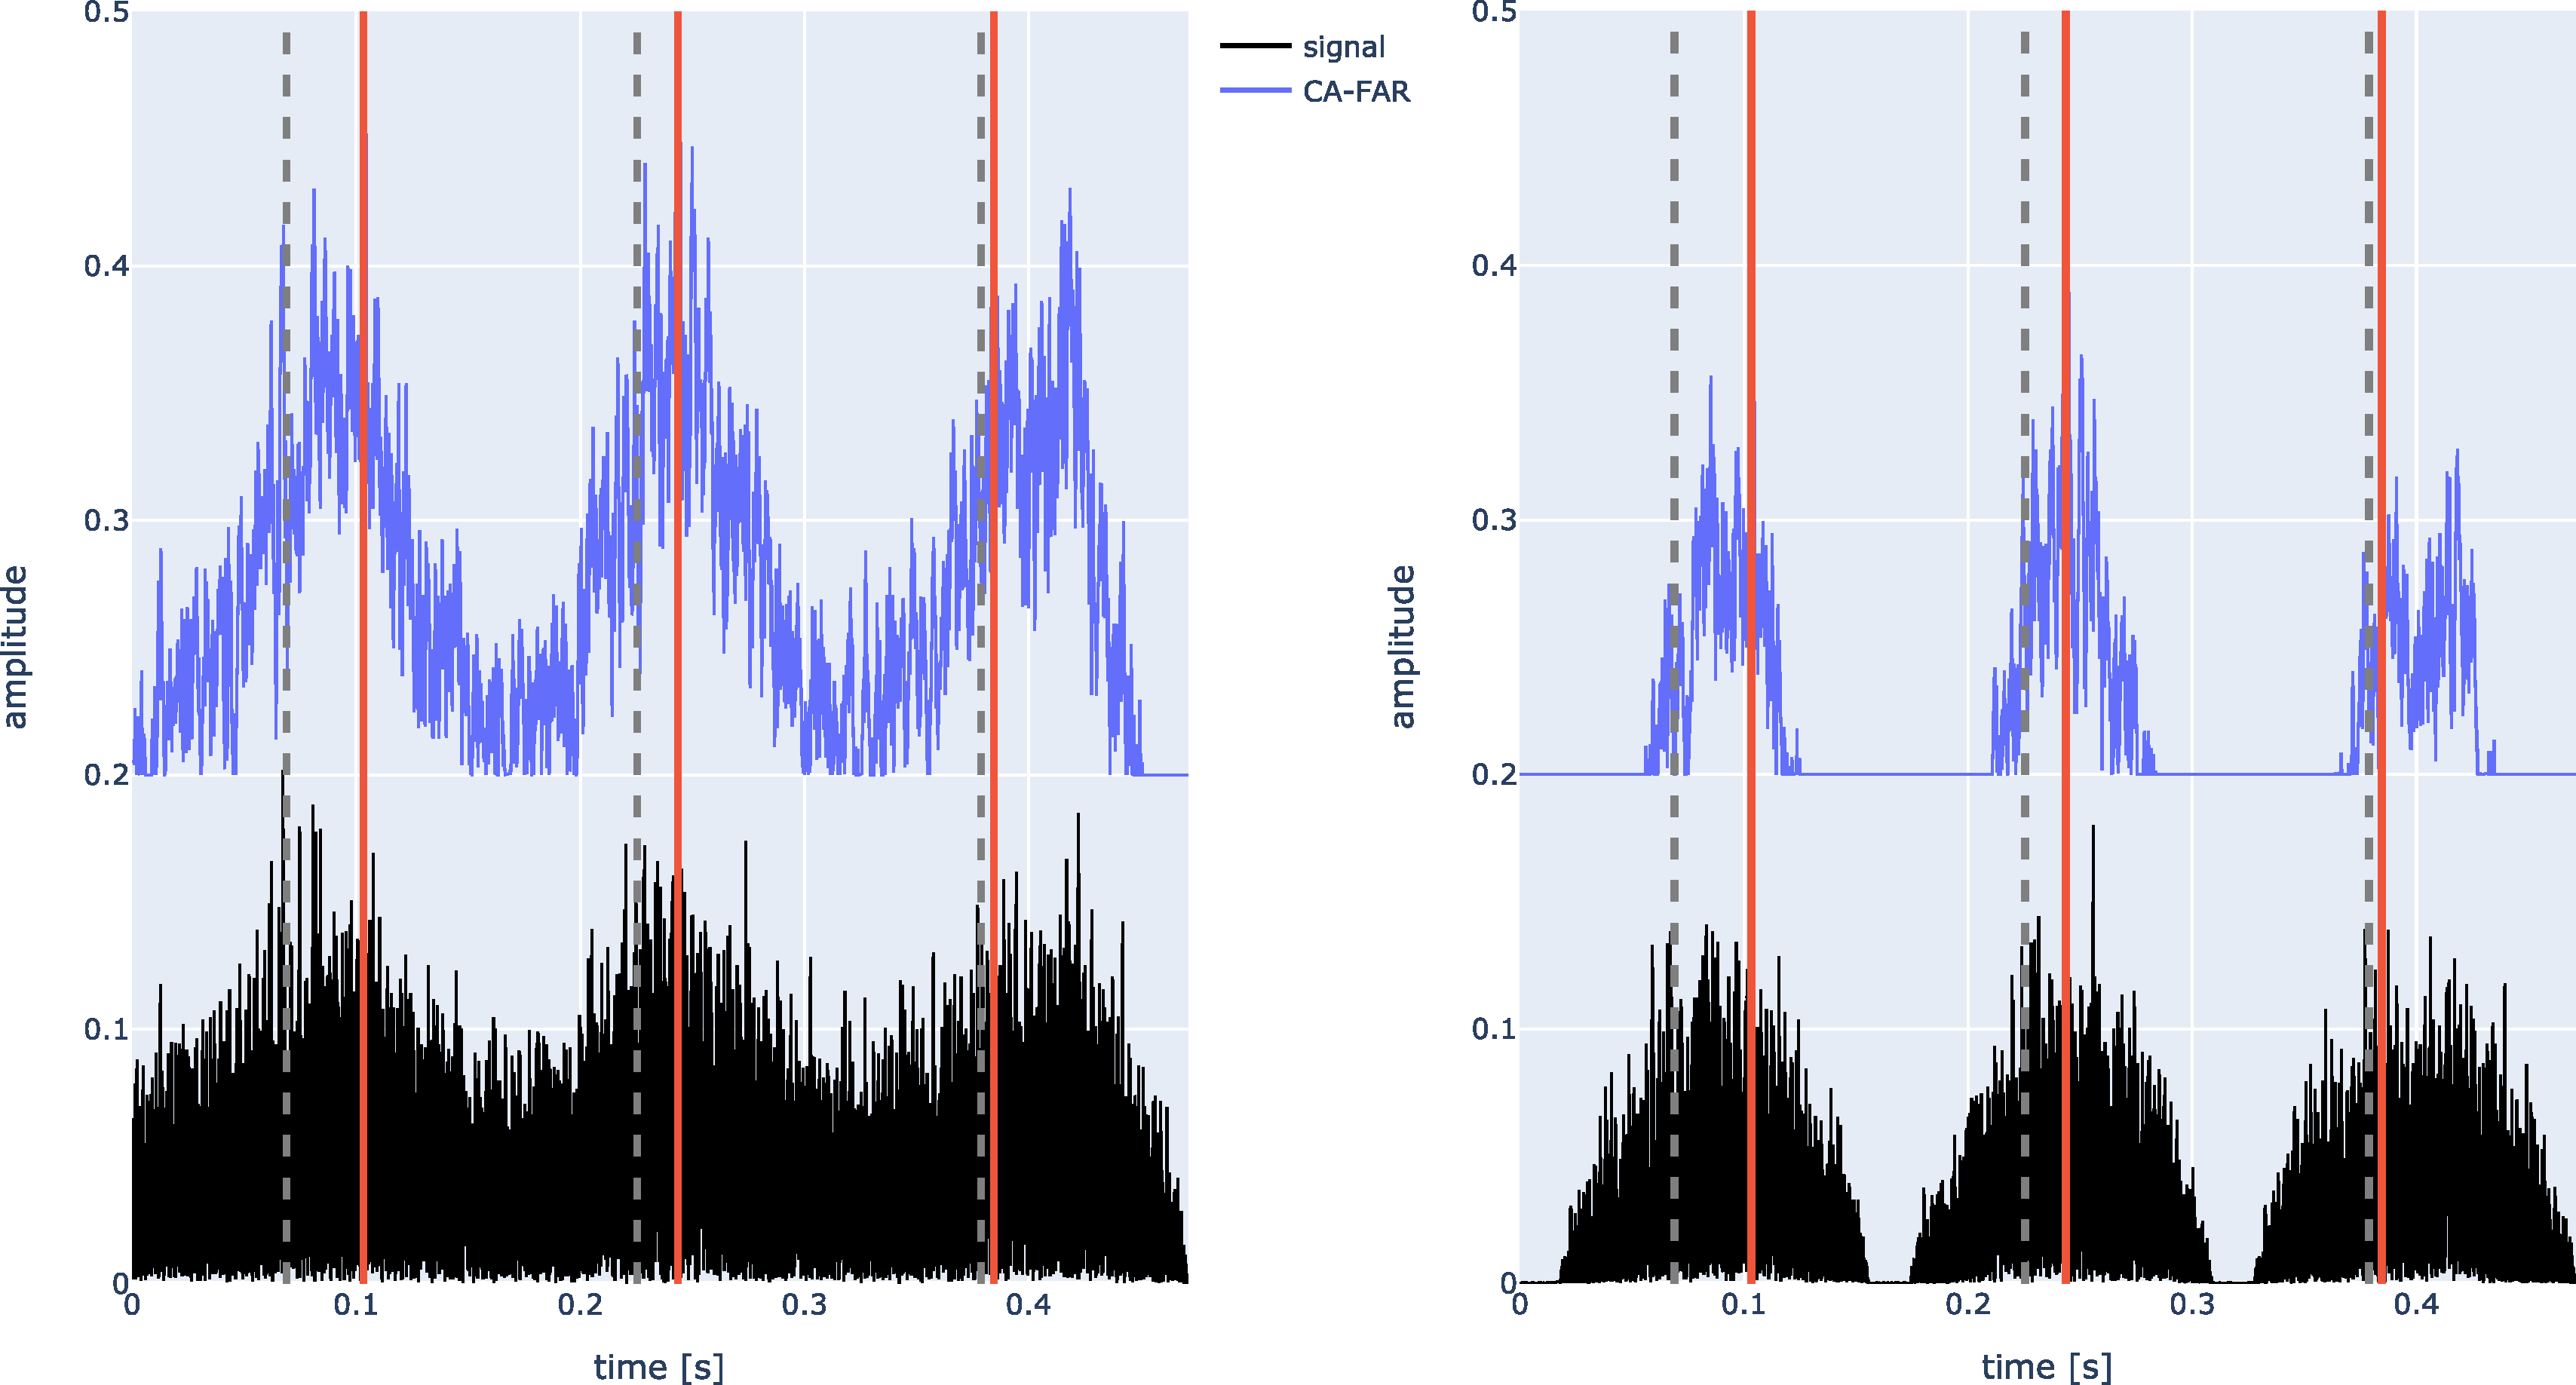
\includegraphics[width=\linewidth]{images/simulation/d10snr-5vs20lines} 
	\caption{Correlation of an anchor for first three positions. The gray dotted line marks the first peak of the period, the red line one of the current correlating anchor.}
	\label{fig:3dvslines1}
\end{figure}
By iterating though SNR's between \SI{-5}{\decibel} and \SI{20}{\decibel} in steps of \SI{1}{\decibel} shows that the mean error, which is the average absolute difference between the calculated and expected positions, increases when the SNR is less than \SI{8}{\decibel} and jumps to even higher levels due to the increasing likelihood of false peak detection \ref{fig:errorsnr}.
\begin{figure}
	\centering
	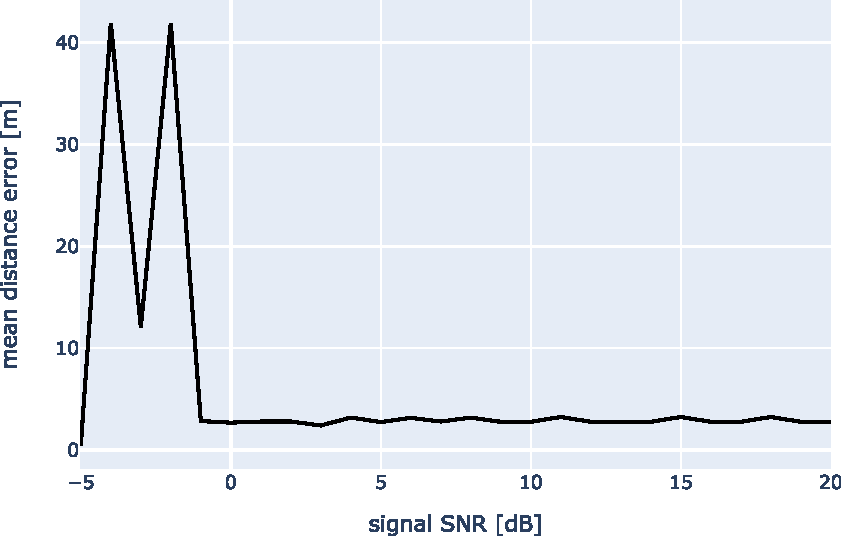
\includegraphics[width=8cm]{images/simulation/snrerror1} 
	\caption{Relationship between SNR and mean distance error}
	\label{fig:errorsnr}
\end{figure}
Continuing with the use of the \SI{-5}{\decibel} SNR the position detection system now incorporates watermark simulations as well. Due to multipath propagation caused by reflections from surfaces, the correlation amplitudes become even higher than those from additive noise \ref{fig:3dvslines2}. As a result, peak detection becomes less reliable, and it becomes necessary to adjust the false alarm rate.
\begin{figure}
	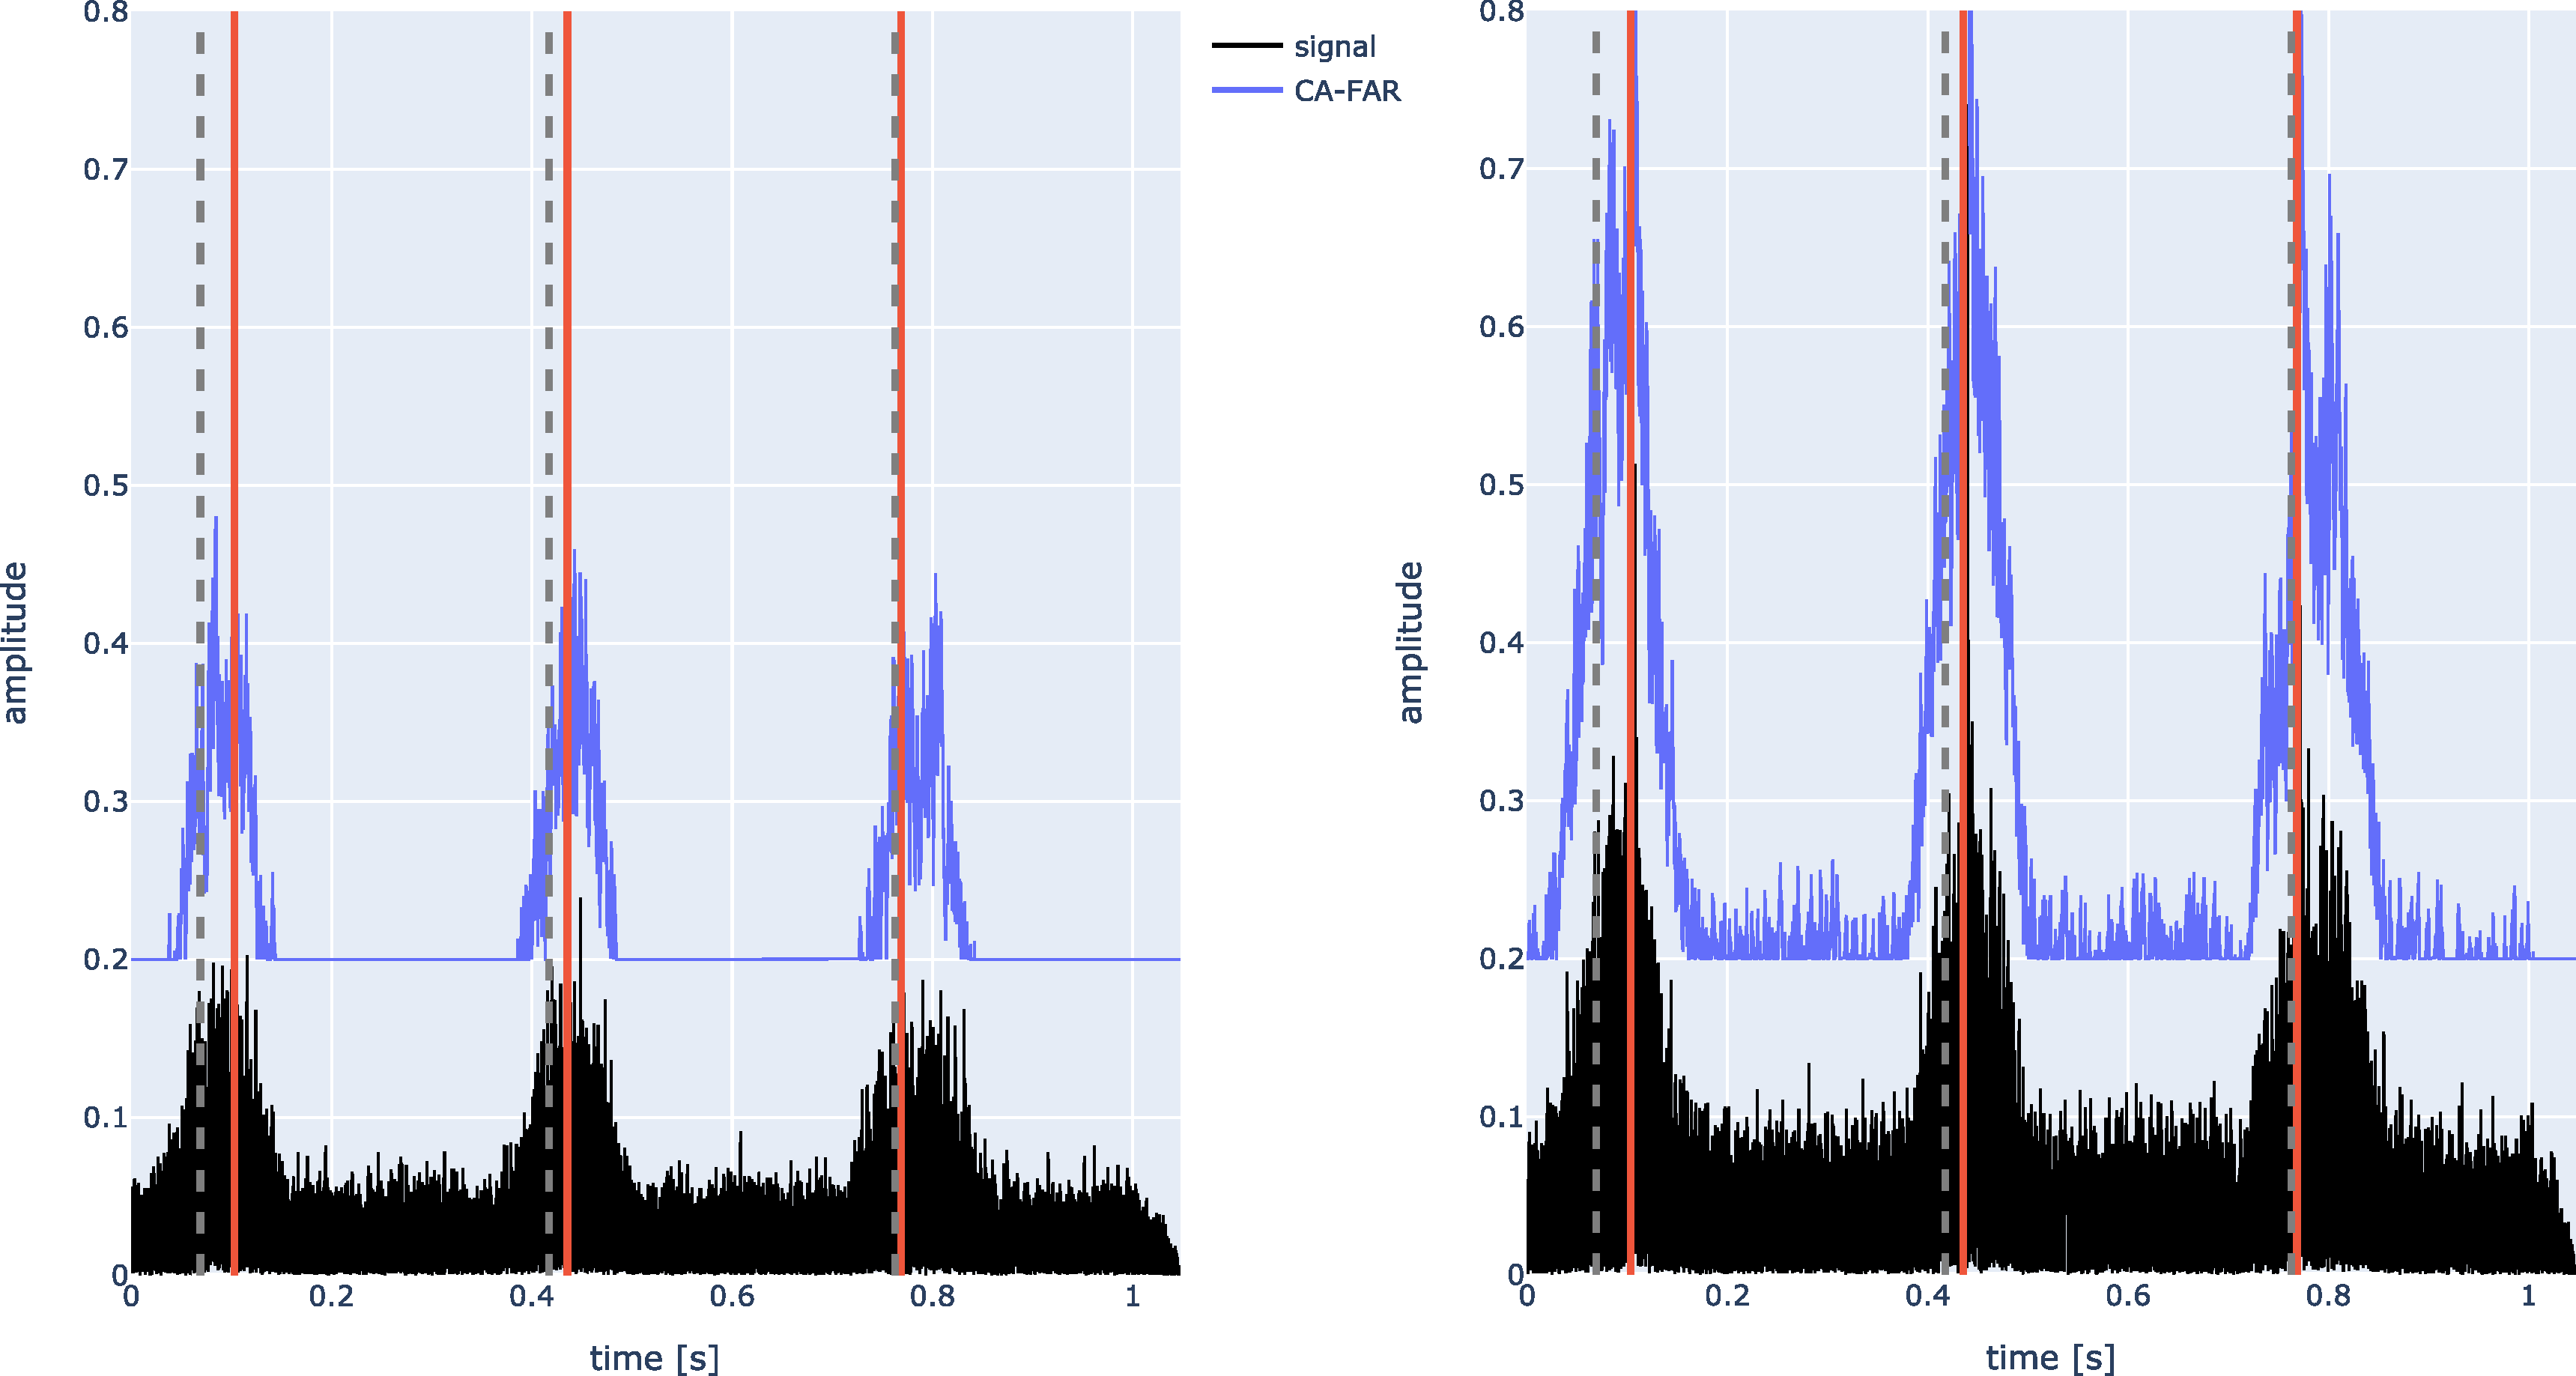
\includegraphics[width=\linewidth]{images/simulation/d10plane1vscastle2lines} 
	\caption{Correlation of an anchor for first three positions using watermark simulation channel PLANE1 at the right and CASTLE2 at the left, both with additive white noise of \SI{-5}{\decibel}}
	\label{fig:3dvslines2}
\end{figure}
\newpage
\section{Localization field testing}
A field test was conducted at a shoreline location. Three hydrophones were deployed at a depth of one meter below sea level. Anchors A and B were positioned with a distance of \SI{4.1}{\meter} between them, with Anchor B located \SI{10.74}{\meter} from the receiving hydrophone. During the test, the underwater speed of sound, as measured using a CTD Sensor (Conductivity, Temperature, and Depth), was \SI{1430.3}{\meter\per\second}. The receiving hydrophone was also relocated to a second location, \SI{5.56}{\meter} from Anchor B.

In the first run codes of degree ten were transmitted for a total time of \SI{50}{\second}. Afterwards the receiving hydrophone was moved \SI{5.18}{\meter} further away from the anchors. Then again three test runs were done with code degrees of ten, nine and seven. Every run was repeated with a more decreased signal intensity for testing lower SNR's.
\begin{figure}
	\centering
	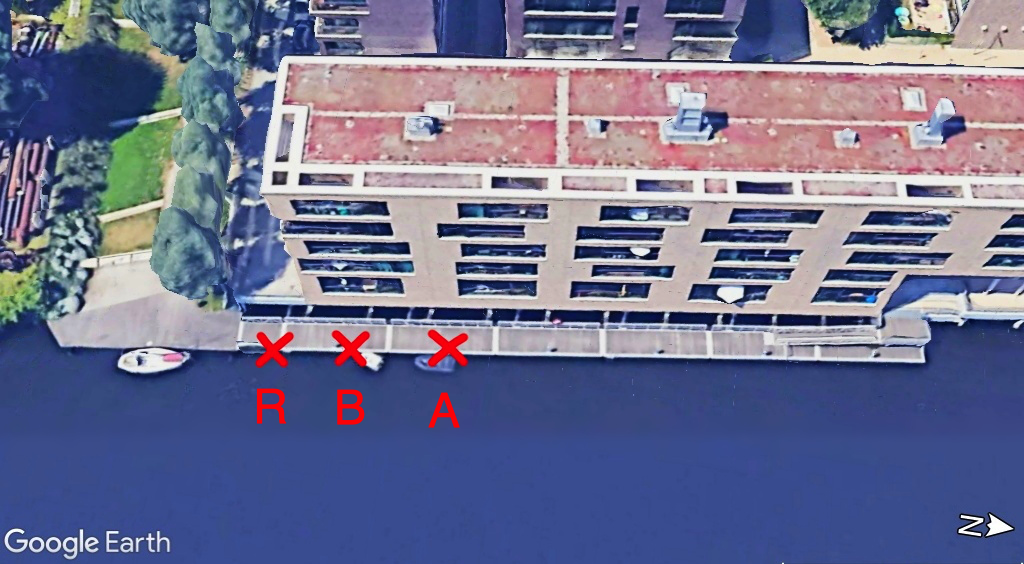
\includegraphics[width=12cm]{images/labloc}
	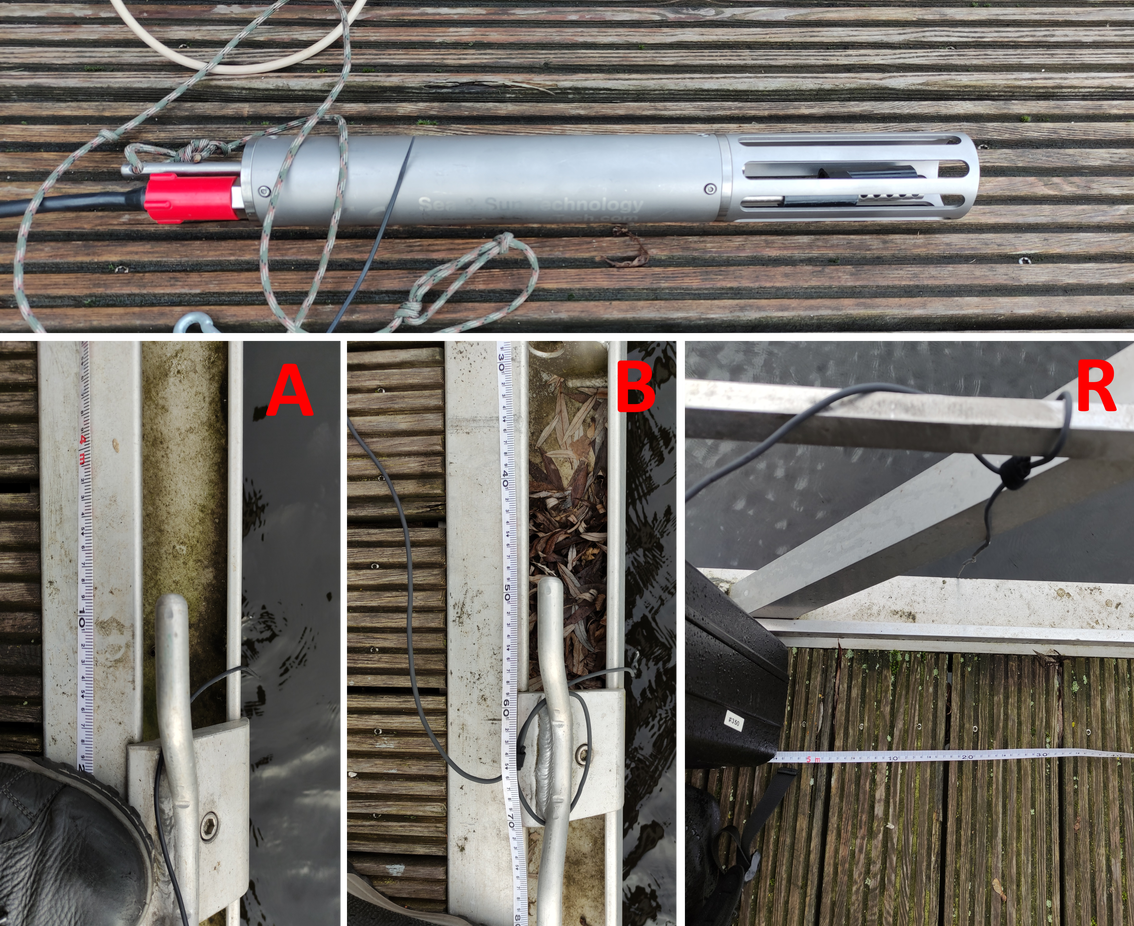
\includegraphics[width=12cm]{images/measurerealcomp}
	\caption{Location of field test, the markings represent the positions of the hydrophones. From left to right: receiver, sending anchor B and A. The CTD Sensor is depicted in the middle.}
	\label{fig:simsig}
\end{figure}
The figures presented here show the measured and expected values of a position over time for a standard and decreased signal strength for all three degrees of code.

\begin{figure}
	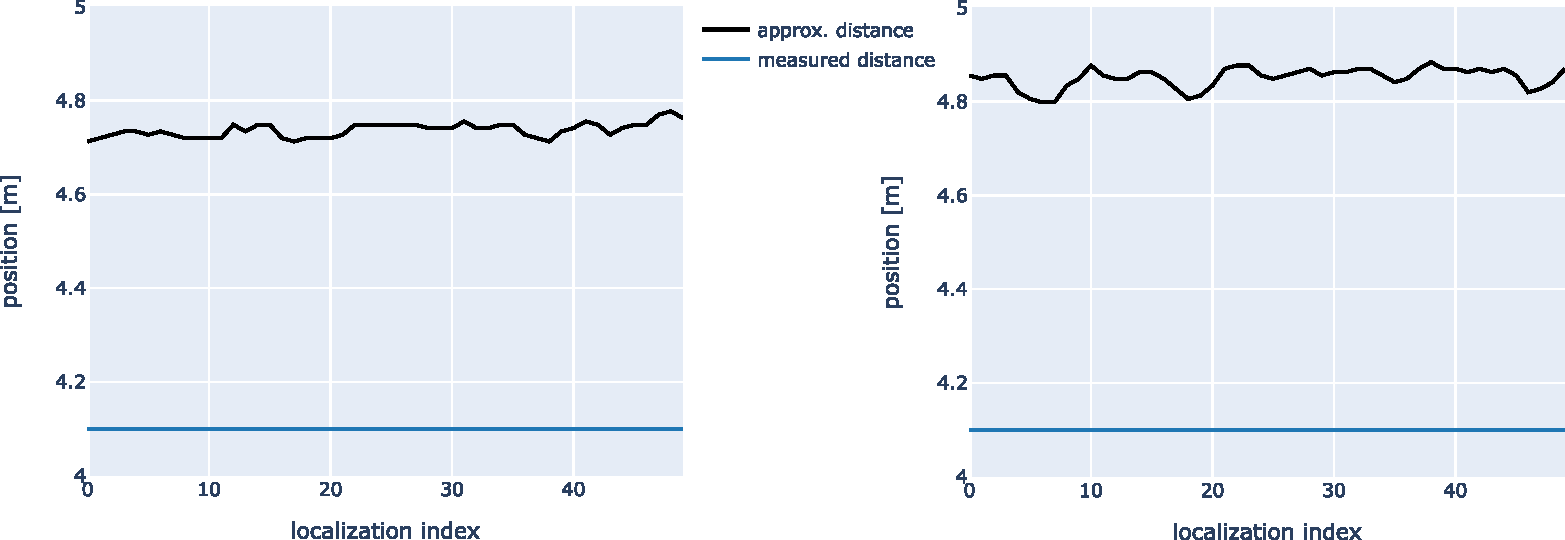
\includegraphics[width=\linewidth]{images/d10fvsd10fn} 
	\caption{Evaluation of 10th degree code. High SNR at the left and low SNR at the right.}
	\label{fig:d10fvsd10fn}
\end{figure}
It is observed that with a code of 10th degree, there is a significant offset of approximately \SI{60}{\centi\meter} between the measured and expected values \ref{fig:d10fvsd10fn}. This offset is likely a result of synchronization problems between the oscilloscopes used in the experiment. However, it is also worth noting that despite this offset, the position demonstrates a high degree of stability with minimal variations of less than \SI{10}{\centi\meter}. Additionally, by decreasing the SNR, it is observed that the position is shifted somewhat by under \SI{20}{\centi\meter}. In conclusion, this demonstrates that despite the offset, the overall position remains relatively consistent.
\begin{figure}
	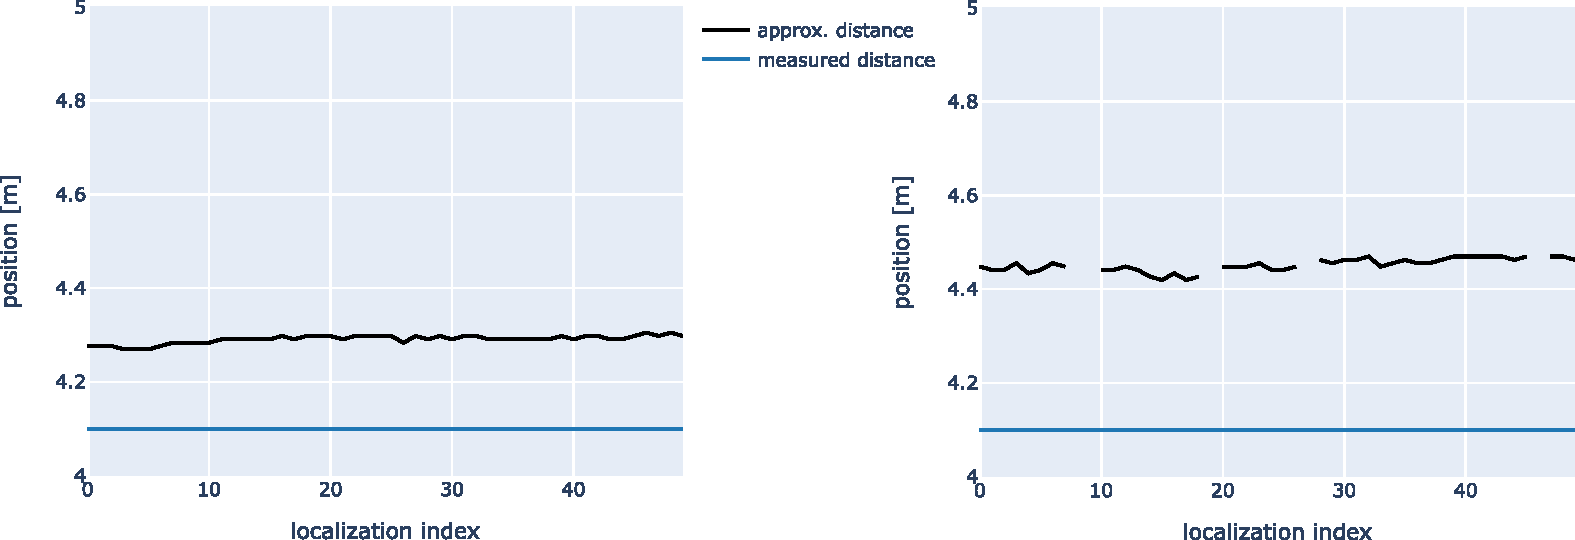
\includegraphics[width=\linewidth]{images/d9fvsd9fn} 
	\caption{Evaluation of 9th degree code}
	\label{fig:d9fvsd9fn}
\end{figure}
The next measure presents the results of the position measurement when the code of 9th degree is used. It is observed that when the default SNR is in use, similar results are obtained as with codes of 10th degree. However, when the SNR is decreased, the peak detection fails \ref{fig:d9fvsd9fn}. This is an important issue to consider, as the ability to accurately detect peaks is crucial for obtaining accurate position measurements. Additionally, values outside the interval from $4$ to $5$ were excluded. The failure of peak detection in this measure is likely due to the enlarged sidelobes, which are known to distract the CFAR algorithm. As a result, the performance of the system is worse compared to when the code is at 10 degrees. This highlights the importance of maintaining a high SNR and the potential impact of sidelobes on the performance of the algorithm.

\begin{figure}
	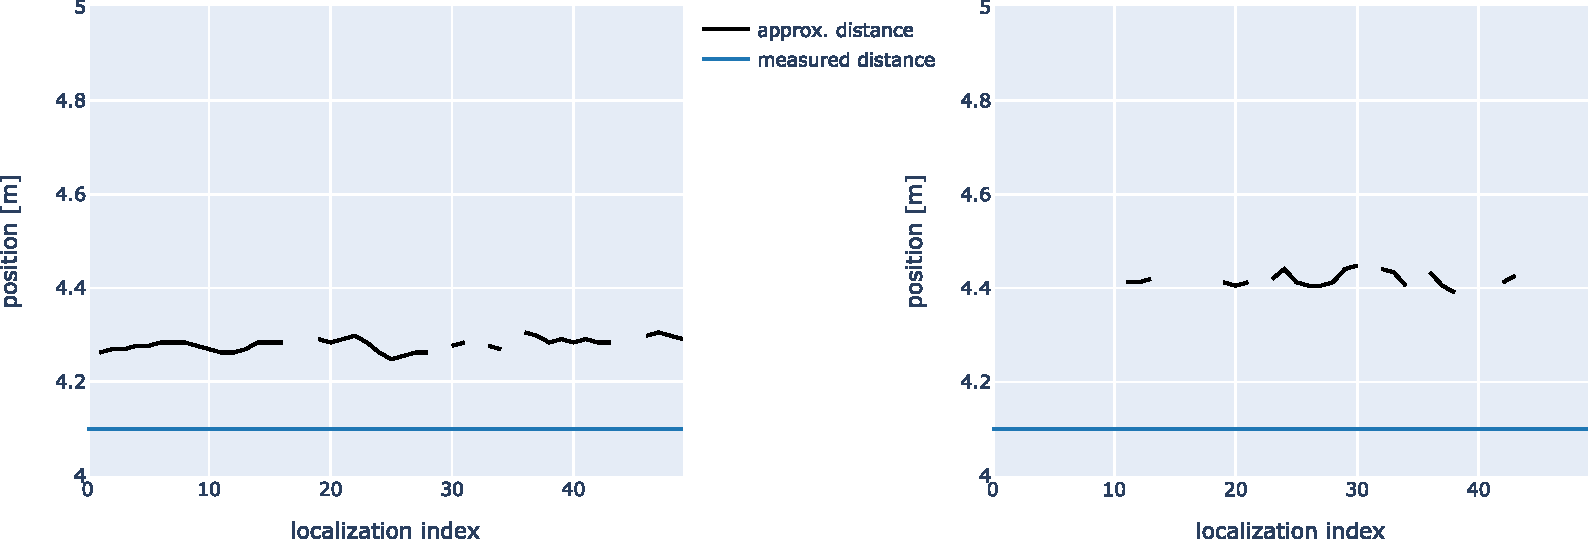
\includegraphics[width=\linewidth]{images/d8fvsd8fn}
	\caption{Evaluation of 8th degree code}
	\label{fig:d8fvsd8fn}
\end{figure}

The final measure presents the results of the position measurement with code of 8th degree. It is observed that this measure follows the downwards trend of performance that was previously noted with code of 9th degree. Specifically, it is found that both low and high SNR position detection's could not be completed without outliers resulting from failed peak detection \ref{fig:d8fvsd8fn}. This further emphasizes the importance of maintaining a high SNR and the potential impact of sidelobes on the performance of the algorithm.

\begin{tuhhtable}
	\centering
	\begin{tabular}[tp]{C{.2\linewidth}C{.2\linewidth}R{.2\linewidth}R{.2\linewidth}}
		\THc{1}{c}{code degree} & \THc{1}{c}{SNR} & \THc{1}{c}{fasle alarm rate} & \THc{1}{c}{minimum theshold} \\
		\abovebodyrule
		10 &  high & 9\% & 0.2 \\\TRc
		10 &  low & 12\% & 0.4 \\
		\hline
		9 &  high & 12\% & 0.2 \\\TRc
		9 &  low & 17\% & 0.4 \\
		\hline
		8 &  high & 26\% & 0.4 \\\TRc
		8 &  low & 26\% & 0.4 \\
		\belowbodyrule
	\end{tabular}
	\caption{Used false alarm rate and minimum threshold in CFAR for different degrees and SNR's}
	\label{tbl:degfarsnr}
\end{tuhhtable}
It is important to note that the false alarm rate and the minimum threshold of the CFAR algorithm must be adjusted to maintain successful peak detection in varying code degrees and SNR levels. As code degree and SNR decrease, the false alarm rate and minimum threshold must be increased to compensate for decreased system performance \ref{tbl:degfarsnr}.

In conclusion, the results of these measures demonstrate the importance of maintaining a high SNR for accurate peak detection and position measurement. As the code degree decreases, the performance of the system worsens, highlighting the need for codes of higher degrees to achieve better results. Additionally, a small shift in position under \SI{20}{\centi\meter} is observable on all results when the SNR is decreased, emphasizing the importance of a high SNR in maintaining the accuracy of the position measurements.
